% poster-exemplo (versão minimalista)
% http://www.vision.ime.usp.br/~jmena/stuff/poster-exemplo/
%
% Sáb Nov 12 16:20:02 BRST 2011
%
% OBSERVAÇÕES:
%  - Este exemplo de poster foi adaptado (em 08/2010) considerando os modelos:
%    (a) https://teamwork.jacobs-university.de:8443/confluence/display/CoPandBiG/LaTeX+Poster
%    (b) http://www.nathanieljohnston.com/2009/08/latex-poster-template/
%
%  - Veja as dimensões dos posters em: 
%    http://www.theinternetprinter.com.au/info/A4_A3_A2_A1_A0_Size_Explained.aspx
%

\documentclass[final]{beamer} 
\usepackage[size=a1, orientation=portrait]{beamerposter} % font scale factor=1.0

\usepackage[brazilian]{babel}
\usepackage[utf8]{inputenc}
\usepackage{lmodern}
\usepackage{clrscode3e}                 % para formatar algoritmos como o CLRS

% cores utilizadas para os algoritmos
\usepackage{framed}
\definecolor{treinamento}{rgb}{0.76471,0.81176,0.91373}  % c3cfe9 -> 195,207,233 -> 0.76471   0.81176   0.91373
\definecolor{reconstrucao}{rgb}{0.83529,0.80784,0.89804} % d5cee5 -> 213,206,229 -> 0.83529   0.80784   0.89804
\definecolor{n_red}{HTML}{D7191C}
\definecolor{n_orange}{HTML}{FD9B61}
\definecolor{n_green}{HTML}{3F745A}
\definecolor{n_green_bg}{HTML}{AAE6C9}
\definecolor{n_blue}{HTML}{2B83BA}
\definecolor{n_violet}{HTML}{AC146D}
\definecolor{n_yellow}{HTML}{D2D221}
\definecolor{RawSienna}{cmyk}{0,0.72,1,0.45}
\definecolor{olive}{rgb}{0.3, 0.4, .1}

\newcommand{\colorize}[2]{\textbf{\textcolor{#1}{#2}}}

\graphicspath{{./figures/}}  
\urlstyle{same}


%==The poster style============================================================
\usetheme{poster-exemplo}            % our poster style
%--set colors for blocks (without frame)---------------------------------------
  \setbeamercolor{block title}{fg=ngreen,bg=white}
  \setbeamercolor{block body}{fg=black,bg=white}
%--set colors for alerted blocks (with frame)----------------------------------
%--textcolor = fg, backgroundcolor = bg, dblue is the jacobs blue
  \setbeamercolor{block alerted title}{fg=white,bg=dblue!70}%frame color
  \setbeamercolor{block alerted body}{fg=black,bg=dblue!10}%body color
%
%==Titel, date and authors of the poster=======================================
\title{Um Algoritmo de Escalonamento para Redução do Consumo de Energia em
Computação em Nuvem}
\author{Pedro Paulo Vezzá Campos \and \\  Orientador: Prof. Dr. Daniel Macêdo Batista}
\institute{Depto. de Ciência da Computação -- Instituto de Matemática e 
Estatística -- Universidade de São Paulo}


%==============================================================================
%==the poster content==========================================================
%==============================================================================
\begin{document}
%--the poster is one beamer frame, so we have to start with:
\begin{frame}[t]
%--to seperate the poster in columns we can use the columns environment
\begin{columns}[t] % the [t] options aligns the columns content at the top
%--the left column-------------------------------------------------------------
%\begin{column}{0.28\paperwidth}% the right size for a 3-column layout
\begin{column}{0.35\paperwidth}% the right size for a 3-column layout

	\begin{alertblock}{Introdução}
		A \colorize{RawSienna}{Lei de Moore}, que profetiza que o poder computacional de dispositivos
		dobra a cada 18 meses, está chegando ao fim da sua vida \cite{lei_moore}.
		Processadores atuais atingiram uma barreira de potência mas no entanto
		não eram eficientes no \colorize{olive}{consumo energético} \cite{barroso}. Assim, novas
		tendências surgiram na indústria: processadores mais simples, mais 
		paralelos e mais eficientes.

		\vskip2ex
		
		\colorize{n_red}{Computação em nuvem} surgiu como uma consequência quase natural destas
		tendências. Ao consolidar poder de processamento, transferência de dados
		e armazenamento é possível reduzir custos e desperdícios. Algumas
		estratégias possíveis: \colorize{n_green}{consolidação} de máquinas virtuais,
		dimensionamento de tensão e frequência (\colorize{n_blue}{DVFS}) e
		\colorize{n_violet}{algoritmos energeticamente eficientes}.
		
		\vskip2ex
		
		Este trabalho apresenta um \colorize{black}{novo algoritmo} de escalonamento de fluxos de
		trabalho em computação em nuvem voltado para a eficiência energética.
		O desempenho foi comparado com o trabalho ``\emph{Energy-aware
		simulation with DVFS}'' \cite{guerout} e com um algoritmo de escalonamento clássico
		mas sem um foco na eficiência energética.
				
	\end{alertblock}

\end{column}

% ---------------------------------------------------------------------------- %
\begin{column}{0.60\paperwidth} 
	\begin{block}{Escalonamento de fluxos de trabalho com computação em nuvem}
		\begin{columns}[totalwidth=0.60\paperwidth]
		\begin{column}{0.28\paperwidth}
		
		Podemos modelar algum processamento paralelo a ser computado como um
		\colorize{RawSienna}{digrafo acíclico} (DAG). Um exemplo, é a aplicação Montage da figura
		abaixo, que produz mosaicos astronômicos. Dúvida: como associar uma
		tarefa a uma máquina de forma a diminuir o tempo de processamento ou
		energia consumida? O problema de achar um
		\colorize{n_blue}{escalonamento} ótimo é \colorize{n_red}{NP-difícil}!
		
		\vskip2ex

		\begin{center}
			\includegraphics[width=0.80\columnwidth]{Montage_PP.png}
		\end{center}

		Um algoritmo clássico e boa heurística para o escalonamento é o
		\emph{Heterogeneous Earliest Finish Time} (HEFT) \cite{heft}.

%		\vskip4ex

%		\definecolor{shadecolor}{named}{treinamento}
%		\begin{shaded}
%		{\footnotesize}
%		\end{shaded}
%
%
%		\definecolor{shadecolor}{named}{reconstrucao}
%		\begin{shaded}
%		{\footnotesize}
%		\end{shaded}

		\end{column}
		\begin{column}{0.28\paperwidth}
			O \colorize{black}{HEFT} é dividido em dois momentos: \colorize{olive}{priorização} e 
			\colorize{n_violet}{seleção}. No primeiro, define quais tarefas
			escalonar primeiro. O segundo aloca cada tarefa em ordem de prioridade
			de maneira a minimizar o tempo mais cedo de conclusão dela.
		
			\begin{center}
				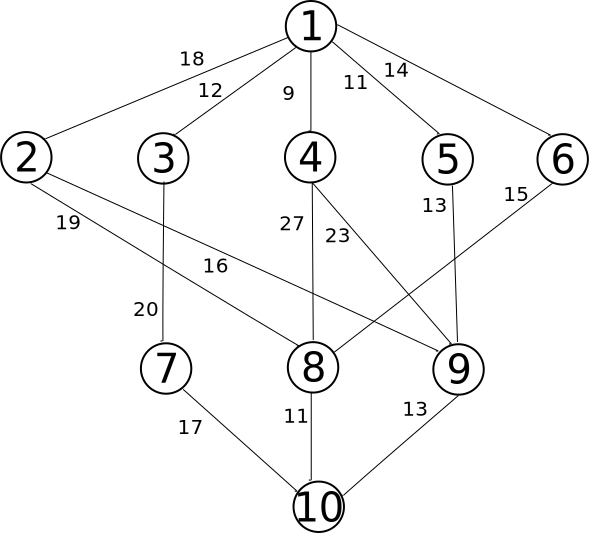
\includegraphics[width=0.70\columnwidth]{dag_heft.pdf}
			\end{center}	

			\begin{center}
				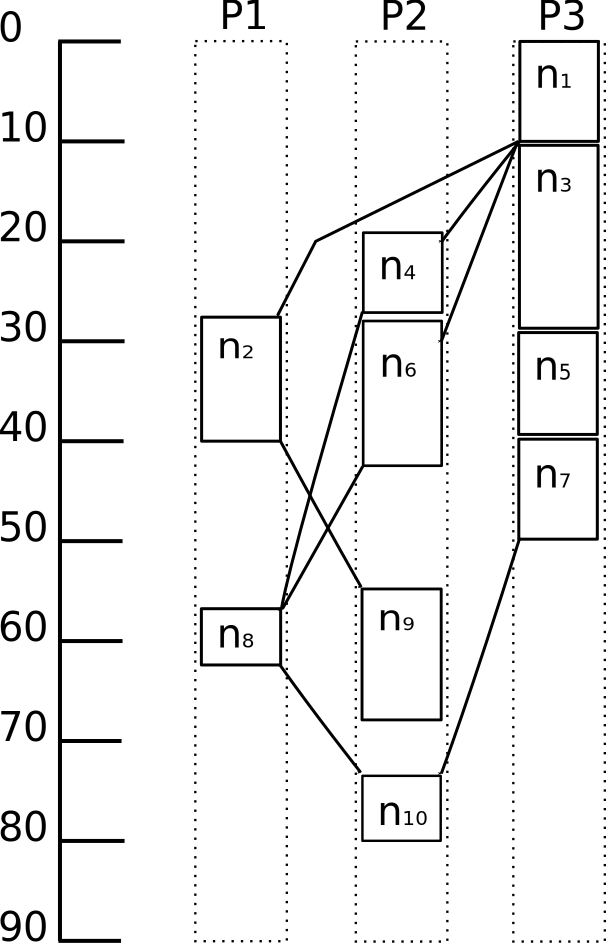
\includegraphics[width=0.40\columnwidth]{escalonamento_heft.pdf}
			\end{center}	
		
		\end{column}
		\end{columns}

	\end{block}
	%\vskip2ex

\end{column}
\end{columns}

\vskip2ex

% ---------------------------------------------------------------------------- %

\begin{columns}[t] 
\begin{column}{0.35\paperwidth}

	\begin{block}{Algoritmo Proposto}
	\begin{codebox}
	\Procname{$PowerHEFTLookahead()$}
		\li $V \gets \{VmMaisRápida\}$ \Comment VMs usadas ao escalonar
%		\li Seja O o conjunto de opçoes de VMs que podem ser instanciadas
%		Ordene o conjunto de tarefas segundo o critério rank\_u
%	   
%		Enquanto há tarefas não escalonadas:
%		    t <- a tarefa não escalonada de maior rank\_u
%		    F <- filhos de t
%		   
%		    //Vamos tentar escalonar t em uma VM já existente
%		    para cada v em V:
%		        Escalone t em v
%		        Escalone todas as tarefas de F utilizando o algoritmo HEFT
%		        Energia\_v <- Uma estimativa energia consumida no escalonamento do passo anterior
%		        Volte para o estado de escalonamento do começo deste laço
%		   
%		    //Vamos tentar escalonar t em uma nova VM
%		    para cada o em O:
%		        V\_novo <- V U {o}
%		        Atualize os valores de rank\_u
%		        t\_novo <- a tarefa não escalonada de maior rank\_u
%		        F\_novo <- filhos de t
%		       
%		        Escalone t\_novo em o
%		        Escalone todas as tarefas de F\_novo utilizando o algoritmo HEFT
%		        Energia\_o <- Uma estimativa energia consumida no escalonamento do passo anterior
%		        Volte para o estado de escalonamento do começo deste laço
%		   
%		    Escalone t na VM que minimiza a energia consumida
%		    Atualize V e rank\_u caso necessário
	\End
	\end{codebox}
	
	
%		\begin{codebox}
%		\Procname{$\proc{Heterogeneous-Earliest-Finish-Time}()$}
%		\li	Defina os custos computacionais das tarefas e os custos\\
%			de comunicação das arestas com valores médios
%		\li	Calcule $rank_u$ para todas as tarefas varrendo o grafo\\
%			de ``baixo para cima'',	iniciando pela tarefa final.
%		\li Ordene as tarefas em uma lista de escalonamento\\
%			utilizando uma ordem não crescente de valores de $rank_u$.
%		\li 	\While há tarefas não escalonadas na lista
%		\li 		\Do
%						Selecione a primeira tarefa, $n_i$ da lista de escalonamento.
%		\li				\For cada processafor $p_k$ no conjunto de processadores $(p_k \in P)$
%		\li 				\Do
%								Calcule o tempo mais cedo de conclusão da tarefa  $n_i$,
%								considerando que ela execute \\em $p_k$
%							\End
%		\li				Defina a tarefa $n_i$ para executar no processador $p_j$ que
%							minimiza o tempo mais\\ cedo de conclusão da tarefa $n_i$.
%					\End
%		\End
%		\end{codebox}
	\end{block}
	
	\vspace{1.0em}

	\begin{block}{MatrUSP na Mídia}
		\begin{itemize}
			\item \textbf{Aluno do IME elabora site para ajudar estudantes na matrícula}
			-- \emph{Jornal do Campus}
			\vskip2ex
			\item Mais de \textbf{1000 likes} no Facebook em três dias
		\end{itemize}
	\end{block}


\end{column}

% ---------------------------------------------------------------------------- %
\begin{column}{0.61\paperwidth} 
\begin{block}{Resultados}
	\begin{center}
		\includegraphics[width=\columnwidth]{matrusp.png}\\
		\hfill\emph{Exemplo: Grade horária de aluno da ESALQ, mais de
		7000 combinações de turmas viáveis}
	\end{center}


\begin{columns}[t] 
	\begin{column}{0.45\columnwidth}
	\end{column}

	\begin{column}{0.45\columnwidth}
	\end{column}
\end{columns}

\vskip2ex


\end{block}

\end{column}
\end{columns}

\begin{columns}[t] 
	\begin{column}{0.35\columnwidth}

		\begin{block}{Agradecimentos}
			O autor gostaria de agradecer a Ramiro Polla pelo código fonte original
			do MatrUFSC e o apoio financeiro da Universidade de São
			Paulo através do programa Ensinar com Pesquisa, que financia o Projeto
			Apoio BCC, do qual o autor é bolsista de iniciação científica.
		\end{block}

	\end{column}

	\begin{column}{0.61\columnwidth}
		\begin{block}{Referências}
			\footnotesize{\begin{thebibliography}{99}
			\bibitem{usp_numeros}
			UNIVERSIDADE DE SÃO PAULO, ``\textbf{USP em Números},'' \emph{Base de dados 2012},
			Disponível em \url{http://www5.usp.br/usp-em-numeros/}. Acesso em 24 de julho de 2013.

			\bibitem{matrufsc}
			R. Polla, ``\textbf{MatrUFSC},'',
			Disponível em \url{http://ramiro.arrozcru.org/matrufsc}. Acesso em 24 de julho de 2013.

			\bibitem{gde}
			F. G. de C. B. Franco , ``\textbf{GDE, a rede de auxílio acadêmico},''
			Disponível em \url{http://grade.daconline.unicamp.br/visoes/Bemvindo.php}. Acesso em 24 de julho de 2013.
			\end{thebibliography}}

		\end{block}
	
	\end{column}
\end{columns}


% ---------------------------------------------------------------------------- %
\end{frame}
\end{document}
